\chapter{Casimir effect}\label{cha:casimir-effect}

Casimir forces can be viewed in a very similar way to the \textit{van der Waals forces}. In fact, both phenomena describe just two different sides of the same coin. They define the so-called \emph{dispersion forces} between neutral atoms or bodies.
The quantum theory of van der Waals forces between two neutral atoms was developed by London in 1930 who found the attractive potential $\propto 1/r^6$ for small separations.
Casimir and Polder showed in 1948, that for separations larger than the resonance wavelength of the atoms, retardation effects need to be taken into account and the potential decays by a power law of $1/r^7$ \cite{Casimir_1948a}. 
Additionally, they calculated the interaction with a atom or molecule and a perfectly conducting wall, showing that macroscopic objects could experience these \emph{Casimir-Polder interactions} as well.
It becomes evident, that a full description of dispersion forces cannot be given by classical electrodynamics alone. Additional considerations regarding relativistic effects and quantum electrodynamics have to be made \cite{Bordag_2001,Klimchitskaya_2009,Lamoreaux_2004}.
Casimir, following a suggestion by Bohr \cite{Bordag_1999}, found a simple derivation using the zero-point energy of the vacuum to calculate the attraction between two conducting plates.
In quantum electrodynamics each point in the electromagnetic field can be described by an quantized harmonic oscillator with ground state energy $E_0 = \hbar\omega/2$.
The total \textit{zero-point energy} of the ground state of the field (the vacuum) is therefore given by summing over the energies $E_0$ for each possible mode $n$
\begin{equation}
  E_\mathrm{vacuum} = \frac{\hbar}{2} \sum_n \omega_n.
\end{equation} 
These sums are clearly divergent since there are infinitely many possible excitations.
Electrostatic boundary conditions require the field to be zero at the surface of the plate restricting the possible modes between the plates.
Precisely the finite difference between the infinite vacuum energy with and without the plates give rise to the \emph{Casimir forces} between two macroscopic objects.
A lot of textbooks are simply dropping the divergence motivated by the fact that energy is normally defined only up to a constant \cite{Bordag_2001}. 
Casimir was able to use regularization techniques to deal with the infinite quantities and arrived at his famous formula \cite{Casimir_1948}
\begin{equation}\label{eq:3:casimir-energy-pp-conducting}
  E_\mathrm{Casimir} = -\frac{\hbar c \pi^2}{720 L^3} A .
\end{equation}
for the attractive Casimir-potential between two plates with area $A$ and separation $L$.
The attractive force between the plates can now be simply expressed as
\begin{equation}\label{eq:3:casimir-force-pp-conducting}
  F_\mathrm{Casimir} = - \frac{\hbar c \pi^2}{240 L^4} A .
\end{equation}
It is remarkable, that such a simple relation arises out of the infinities of the vacuum.
Up until now, these Casimir forces are topic of modern scientific research. They are generally very difficult to calculate for other geometries than two infinitely large plates or for real materials with dielectric properties. 
Even for simple geometries, even the sign of the force is not always intuitively clear: As an example, the Casimir force can be repulsive for an ideal metal spherical shell \cite{Klimchitskaya_2009}.
For other simple and important bodies like the sphere-plane or sphere-sphere geometry, no universally valid formula for any separation between the bodies exists. This is discussed in more detail in \cref{sec:3:sphere-plate}.

Almost ten years after the discovery of Casimir and Polder, Lifshitz was the first to find an expression for the Casimir force between two dielectric plates with arbitrary relative permittivity $\varepsilon_{r,\,1,2}$ for separations larger than the resonant wavelength \footnote{The \q{resonance wavelength} for a macroscopic body in this case can be understood as e.g. the plasma frequency in the Drude model \cite{Ford_1998}. Different models for light-matter interaction result in slightly different resonant wavelength. The Lifshitz formula however holds true for the cases of separations in the micro-meter regime for all practical materials \cite{Kamp_2020}.} \cite{Lifshitz_1956}.
The expression he found facilitates the general complexity of the Casimir interactions and is only expressible as a complicated integral \cite{Lifshitz_1956}
\begin{multline}\label{eq:3:lifshitz-general-integral}
  F/A = -\frac{\hbar c}{32 \pi^2 L^4} \int_0^\infty \dd x \int_1^\infty \dd p \ \frac{x^3}{p^2}\biggl\{ \left[ \frac{(s_1+p)(s_2+p)}{(s_1-p)(s_2-p)} e^x - 1 \right]^{-1} + \\
  \left[ \frac{(s_1+ \varepsilon_{r,\,1} p)(s_2 + \varepsilon_{r,\,2} p)}{(s_1 - \varepsilon_{r,\,1} p)(s_2 - \varepsilon_{r,\,2} p)} e^x - 1 \right]^{-1} \biggr\}
\end{multline}
with
\begin{equation*}
  s_{1,2} = \sqrt{\varepsilon_{r,\,1,2} - 1 + p^2} .
\end{equation*}
In the limit of two perfectly conducting plates ($\varepsilon_{r,\,1} = \varepsilon_{r,\,2} \rightarrow \infty$), the integral can be solved analytically and one gets the same expression already obtained by Casimir
\begin{equation}
  F_\mathrm{cond.}/A = -\frac{\hbar c}{16 \pi^2 L^4} \int_0^\infty \dd x \int_1^\infty \dd p \ \frac{x^3}{p^2 (e^x - 1)} = -\frac{\hbar c \pi^2}{240 L^4} .
\end{equation}
Lifshitz determined the Casimir force between a conducting metal plate and a dielectric plate (denoted $\mathrm{DM}$) as well as the force between two dielectric plates with the same dielectric constant $\varepsilon_r$ ($\mathrm{DD}$) as
\begin{align} \label{eq:3:casimir-pp-F-DM-lifshitz}
  F_\mathrm{DM} &= -\frac{\hbar c \pi^2}{240 L^4} \frac{\varepsilon_r - 1}{\varepsilon_r + 1} \varphi(\varepsilon_r) \\
  F_\mathrm{DD} &= -\frac{\hbar c \pi^2}{240 L^4} \left( \frac{\varepsilon_r - 1}{\varepsilon_r + 1} \right)^2 \varphi(\varepsilon_r)\label{eq:3:casimir-pp-F-DD-lifshitz}
\end{align}
where $\varphi(\varepsilon_r)$ is a numerical function obtained by solving eq. \eqref{eq:3:lifshitz-general-integral}, which approaches $1$ for a perfect conductor. I calculated the function numerically and the result is shown in \cref{fig:3:lifshitz-function}.
\begin{figure}[!htbp]
  \centering
  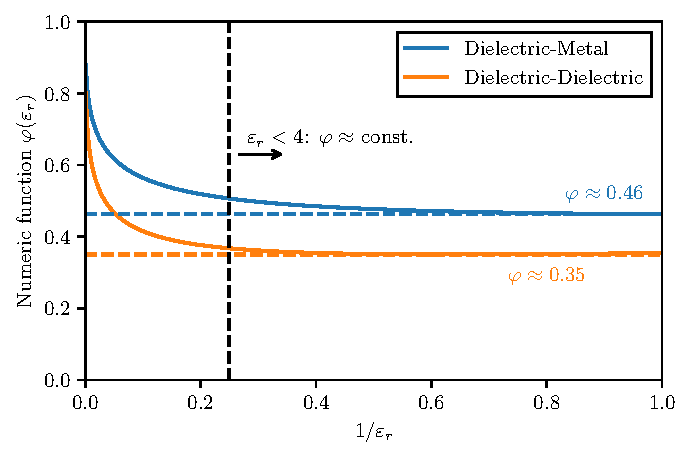
\includegraphics[width=0.8\textwidth]{./../figures/casimir-lifshitz-function.pdf}
  \caption{Numeric calculations of the function $\varphi(\varepsilon)$ used in the Lifshitz formula eq. \eqref{eq:3:casimir-pp-F-DM-lifshitz} and \eqref{eq:3:casimir-pp-F-DD-lifshitz}. The function was calculated for \textbf{(blue)} a dielectric and a metal plates and \textbf{(orange)} two dielectric plates. The function approaches unity for $\varepsilon\rightarrow\infty$ and a finite value for $\varepsilon\rightarrow 1$.}
  \label{fig:3:lifshitz-function}
\end{figure}
For a dielectric and metal plate, the function $\varphi$ approaches the finite value $\varphi(\varepsilon_r \rightarrow 1) \approx 0.46$ for small dielectric constants. However, this limit is practically already reached at $\varepsilon_r \approx 4$ and $\varphi$ stays approximately constant for smaller $\varepsilon_r$.



\section{Proximity force approximation}
\label{sec:3:pfa}

The Casimir-Polder force cannot be computed easily for different shapes. There even exists no analytic expression for the simple (and for this thesis relevant) plate-sphere geometry for all ratios $L/R$ and plate-sphere separations.
For a general shape, even the sign of the force, i.e. whether it is attractive or repulsive, is often unknown.
Fortunately, approximation methods exist and in particular the \emph{proximity-force-approximation (PFA)} can be calculated very easily \cite{Hartmann_2018,Emig_2007a,Bulgac_2006}.
The PFA is only valid for small separations ($L/R \approx 1$) between the considered smooth bodies.
The idea of this approximation is to divide the surfaces of the two bodies into infinitesimal small parallel plates with area $\dd A$ and summing over the forces $\dd F$ (or the Casimir-energy $\dd E$) between them (see \cref{fig:3:PFA}):
\begin{equation}\label{eq:3:pfa}
  E_\mathrm{PFA} = \iint_A \dd A \, \frac{E_\mathrm{plate-plate}}{A}
\end{equation}
where for the casimir energy per unit area $E_\mathrm{plate-plate}/A$ either eq. \eqref{eq:3:casimir-energy-pp-conducting} or any of the Lifshitz equations \eqref{eq:3:casimir-pp-F-DD-lifshitz}, \eqref{eq:3:casimir-pp-F-DM-lifshitz} can be chosen.
\begin{figure}[!htbp]
  \centering
  \def\svgwidth{0.55\textwidth}
  \input{./../figures/proximity-force-approximation.pdf_tex}
  \caption{In the proximity force approximation the sphere is divided into infinitesimal plane areas $\dd A$ which all exert a force $\dd F$ according to eq. \eqref{eq:3:casimir-force-pp-conducting}. All the contributions are added up together.}
  \label{fig:3:PFA}
\end{figure}
For the following calculations, it is important to distinguish between the distance between the plates center and the spheres center $L$ (like used before) and the edge-to-edge distance $\mathscr{L} = L - R$.

The problem with this approximation is, that it is ambiguous, what surface the area element $\dd A$ represents. For the plate-sphere geometry, the element can be either chosen tangential to the sphere or parallel to the plate (or in theory any other fictitious surface somewhere in between) \cite{Bulgac_2006}.
For the plate-sphere geometry, in the limit of the validity of the PFA $\mathscr{L} \ll R$ both methods yield the same result.
For the following calculations, I choose $\dd A$ parallel to the plate and the area can be parameterized with $r\in [0, R]$ and $\varphi \in [0, 2\pi]$ resulting in a distance $z$ between the infinitesimal area elements $z(r) = \mathscr{L} + R - \sqrt{R^2 - r^2}$ \footnote{Taking $\dd A$ tangential to the sphere, it can be parameterized with $\theta \in [0, \pi/2]$ and $\varphi \in [0, 2\pi]$ resulting in $z(\theta) = \mathscr{L} + R - R\cos\theta$. The PFA eq. \eqref{eq:3:pfa} yields with $\dd A = R^2\sin\theta\dd\theta\dd\varphi$ the result $\propto \frac{\pi R^2(R + 2\mathscr{L})}{\mathscr{L}^2(R+\mathscr{L})^2}$ which in the limit of $\mathscr{L} \ll R$ results in the same expression as eq. \eqref{eq:3:PFA-sphere-plate}.}. The PFA eq. \eqref{eq:3:pfa} then yields for a dielectric sphere against a perfectly conducting plate
\begin{align}
  E_\mathrm{plate-sphere} &= -\frac{\hbar c \pi^2}{720} \left(\frac{\varepsilon_r - 1}{\varepsilon_r + 1}\right) \varphi(\varepsilon_r) \int_0^R \dd r \int_0^{2\pi} r\dd \varphi \frac{1}{z(r)^3} \\
  &= -\frac{\hbar c \pi^3}{360} \left(\frac{\varepsilon_r - 1}{\varepsilon_r + 1}\right) \varphi(\varepsilon_r) \frac{R^2}{2\mathscr{L}^2(R + \mathscr{L})} \\
  &\approx -\frac{\hbar c \pi^3}{720} \left(\frac{\varepsilon_r - 1}{\varepsilon_r + 1}\right) \varphi(\varepsilon_r) \frac{R}{\mathscr{L}^2} \label{eq:3:PFA-sphere-plate}
\end{align}



\section{Imperfect plate and spheres}

Python numerical approach, gaussian modes (vibration modes of a spherical plane), perlin noise



\section{Casimir forces between a conducting plate and a dielectric sphere}
\label{sec:3:sphere-plate}

\subsection{Polarizability of a dielectric sphere}
The polarizability $\alpha$ is defined via
\begin{equation}
  \vec{E_\infty} \alpha = \vec{p},
\end{equation}
where $\vec{p}$ is the induced dipole moment and $\vec{E_\infty}$ is the external electric field that induces the dipole moment. For a linear and uniform dielectric, it is given as $\vec{p} = \mathcal{V} \varepsilon_0 (\varepsilon_r - 1) \vec{E_\mathrm{in}}$ \cite[p. 220-226]{Griffiths_2018}. Here, $\mathcal{V}$ is the volume of the object and $\vec{E_\mathrm{in}}$ is the electric field inside the dielectric.
The electrostatic boundary conditions for the problem are given by
\begin{equation}
  V_\mathrm{in} \big|_{r=R} = V_\mathrm{out} \big|_{r=R} 
  \quad \text{and} \quad 
  \varepsilon_r\varepsilon_0\pdv{V_\mathrm{in}}{r}\bigg|_{r=R} = \varepsilon_0\pdv{V_\mathrm{out}}{r} \bigg|_{r=R}
\end{equation}
and the electric potential outside of the sphere at $r\rightarrow\infty$ should be equal to the external dipole-inducing field $V_\mathrm{out} |_{r\rightarrow\infty} = -\vec{E_\infty} \cdot \vec{r} = -E_\infty r\cos\theta$.
The electric potential inside and outside the sphere can be calculated using the spherical decomposition of the general electric potential $V \propto 1/\abs{\vec{r} - \vec{r'}}$ into Legendre Polynomials $P_l$ \cite[p. 188-190]{Griffiths_2018}:
\begin{align}
  V_\mathrm{in}(r, \theta) &= -E_\infty r\cos\theta + \sum_{l=0}^{\infty} A_l r^l P_l(\cos\theta), \\
  V_\mathrm{out}(r, \theta) &= -E_\infty r \cos\theta + \sum_{l=0}^{\infty} \frac{B_l}{r^{l+1}} P_l(\cos\theta).
\end{align}
Applying both boundary conditions, it follows that \cite[p. 249-251]{Griffiths_2018}
\begin{equation}
  \begin{cases}
    A_l = B_l = 0 & \text{for } l \neq 1, \\
  A_1 = -\frac{3}{\varepsilon_r + 2}E_\infty, \quad B_1 = \frac{\varepsilon_r-1}{\varepsilon_r + 2}R^3E_\infty
  \end{cases}
\end{equation}
and the resulting  homogenous electric field $\vec{E_\mathrm{in}} = -\vec{\nabla} V_\mathrm{in}$ inside the sphere is given as
\begin{equation}
  \vec{E_\mathrm{in}} = \frac{3}{\varepsilon_r + 2} \vec{E_\infty} .
\end{equation}
The field is shown on the right in \cref{fig:dielectric-sphere-field}.The polarizability $\alpha$ of the sphere can be now be determined to
\begin{equation}
  \alpha_\mathrm{sphere} = 4\pi \varepsilon_0 R^3 \left(\frac{\varepsilon_r - 1}{\varepsilon_r + 2}\right).
\end{equation}

% \begin{figure}[!htbp]
%   \centering
%   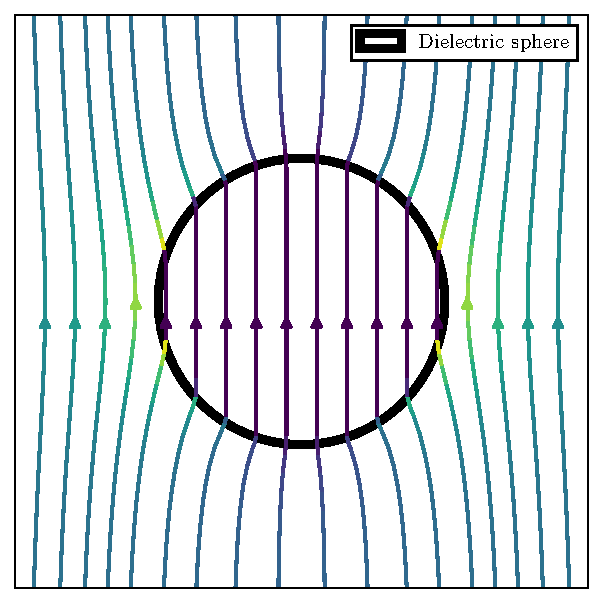
\includegraphics[width=0.8\textwidth]{./../figures/field-dielectric-sphere.pdf}
%   \label{fig:field-dielectric-sphere}
%   \caption{Electric field lines through an dielectric sphere}
% \end{figure}

\begin{figure}[!htbp]
  \centering
  \begin{subfigure}[b]{0.48\textwidth}
      \centering
      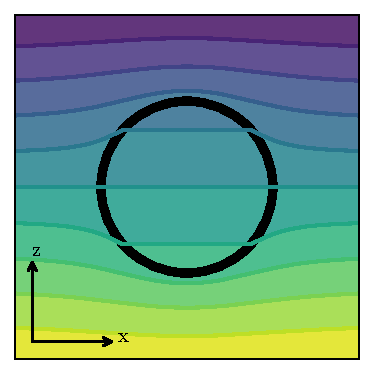
\includegraphics[width=\textwidth]{./../figures/potential-dielectric-sphere-small.pdf}
  \end{subfigure}
  \hfill
  \begin{subfigure}[b]{0.48\textwidth}
      \centering
      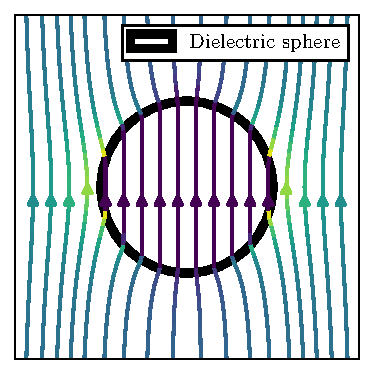
\includegraphics[width=\textwidth]{./../figures/field-dielectric-sphere-small.pdf}
  \end{subfigure}
  \caption{\textbf{left:} Electric potential $V$ of a dielectric sphere in a external electric field $\vec{E_\infty} \parallel \vec{e_z}$. \textbf{right:} The corresponding electric field lines inside and outside the dielectric sphere.}
  \label{fig:dielectric-sphere-field}
\end{figure}